\chapter{Literature Review}



In an time of austerity and double dips in the economy, \gls{IB} is playing `the game' not only over products and customers but also with institutions. Companies like Apple and Samsung are  fighting in court over\gls{IP} in a multitude of countries. The cell phone department of Motorola was bought by Google solely because of it's numerous \glspl{IP}. The field not limited to \glspl{IP}. Next to the fight over \gls{IP} subsidies are at the forefront of the public debate as well. Boeing and Airbus have been fighting over subsidies for decades where on more than one occasion the \gls{WTO} has ruled on the validity of these subsidies. More recently solar panels have become a topic of tariffs between the European Union and China. \\

The field of play is governed by governments, trade blocks and the \gls{WTO} on the one hand and \gls{IB} on the other.
A multitude of forces are acting on this playing field and the different actors on this pitch have to cooperate. 
Different \gls{MNE} will cope differently with the challenges that are set by the institutions and the environment that they are operating in. That this environment is of importance is explained by \gls{IBV}~\cite{Kostova:1999,Meyer:2009,Wang:2012} 

\section{\glsdesc{IBV}}

Using the examples of Google, Apple, Samsung, Boeing and Airbus strategies of the large \mne have extended. It is no longer just resources and industries that dictate the strategies that companies employ. According to \cite{Peng:2009}, the market-based institutional framework has been taken for granted, and formal institutions (such as laws and regulations) and informal institutions (such as cultures and norms) have been assumed away as ``background''.

This trent has given rise to what \cite{Peng:2009} calls the `third leg' of the strategy tripod. \Gls{IBV} has been an addition to the theoris of~\gls{RBV} introduced by~\cite{Barney:1991} and industry based view by \cite{Porter:1980}. 
Since being introduced by \cite{Porter:1980} (Industry based view) and \cite{Barney:1991}(~\gls{RBV}) strategic management (theory) or strategy in short, has gained a lot of momentum in the international business community. 
%The aforementioned article has received more than 5000 citations
%\footnote{according to Google Scholar
 %(http://scholar.google.nl/scholar?cites=3429746403909254791&as_sdt=2005&sciodt=0,5&hl=nl)
%} 
\\ 

The industry based view is known for the five forces (see figure \ref{fig:5forces}), which states that choosing the correct industry is the key to gaining competitive advantage. The competitiveness of a firm is determined by the five \emph{external} forces.

\begin{figure}[htbp] 
	\centering
	\includegraphics[width=0.7\textwidth]{5forces}
 	\caption{Five Forces from \cite{Porter:1980}}
	\label{fig:5forces}
\end{figure}

\Gls{RBV} came as a response to \cite{Porter:1980} a decade later.~\Gls{RBV} argued that a firms strategic advantage is depended on it's heterogeneous resources (a bundle of all assets, knowledge, and capabilities) which have to be
\begin{enumerate}[(a)]
\item must be valuable, in the sense that it exploit opportunities and/or neutralises threats in a firm’s environment
\item must be rare among a firm’s current and potential competition, 
\item must be imperfectly imitable
\item  there cannot be strategically equivalent substitutes for this resource that are valuable but neither rare or imperfectly imitable 
\end{enumerate} 
This concept is also known under the acronym VRIN. In contrast to \gls{InBV} the theory of '\cite{Barney:1991} is \emph{extrospective}. 
\\

In contrast to~\gls{RBV}, which in introspective in nature and \gls{InBV} is extrospective.~\ibv~takes into 
account not only strategic choices driven by industry conditions and firm\-specific resources that 
traditional strategy research emphasises (~\cite{Porter:1980},~\cite{Barney:1991}), but are also a 
reflection of the formal and informal constraints of a particular institutional framework that decision
makers confront (~\cite{Oliver:1997,Scott:1995}). These institutions are influencing the decision making process in~\gls{IB}.  The dynamic that takes place is depicted in picture \ref{fig:ibv}. 

\begin{figure}[htbp!] 
	\centering
	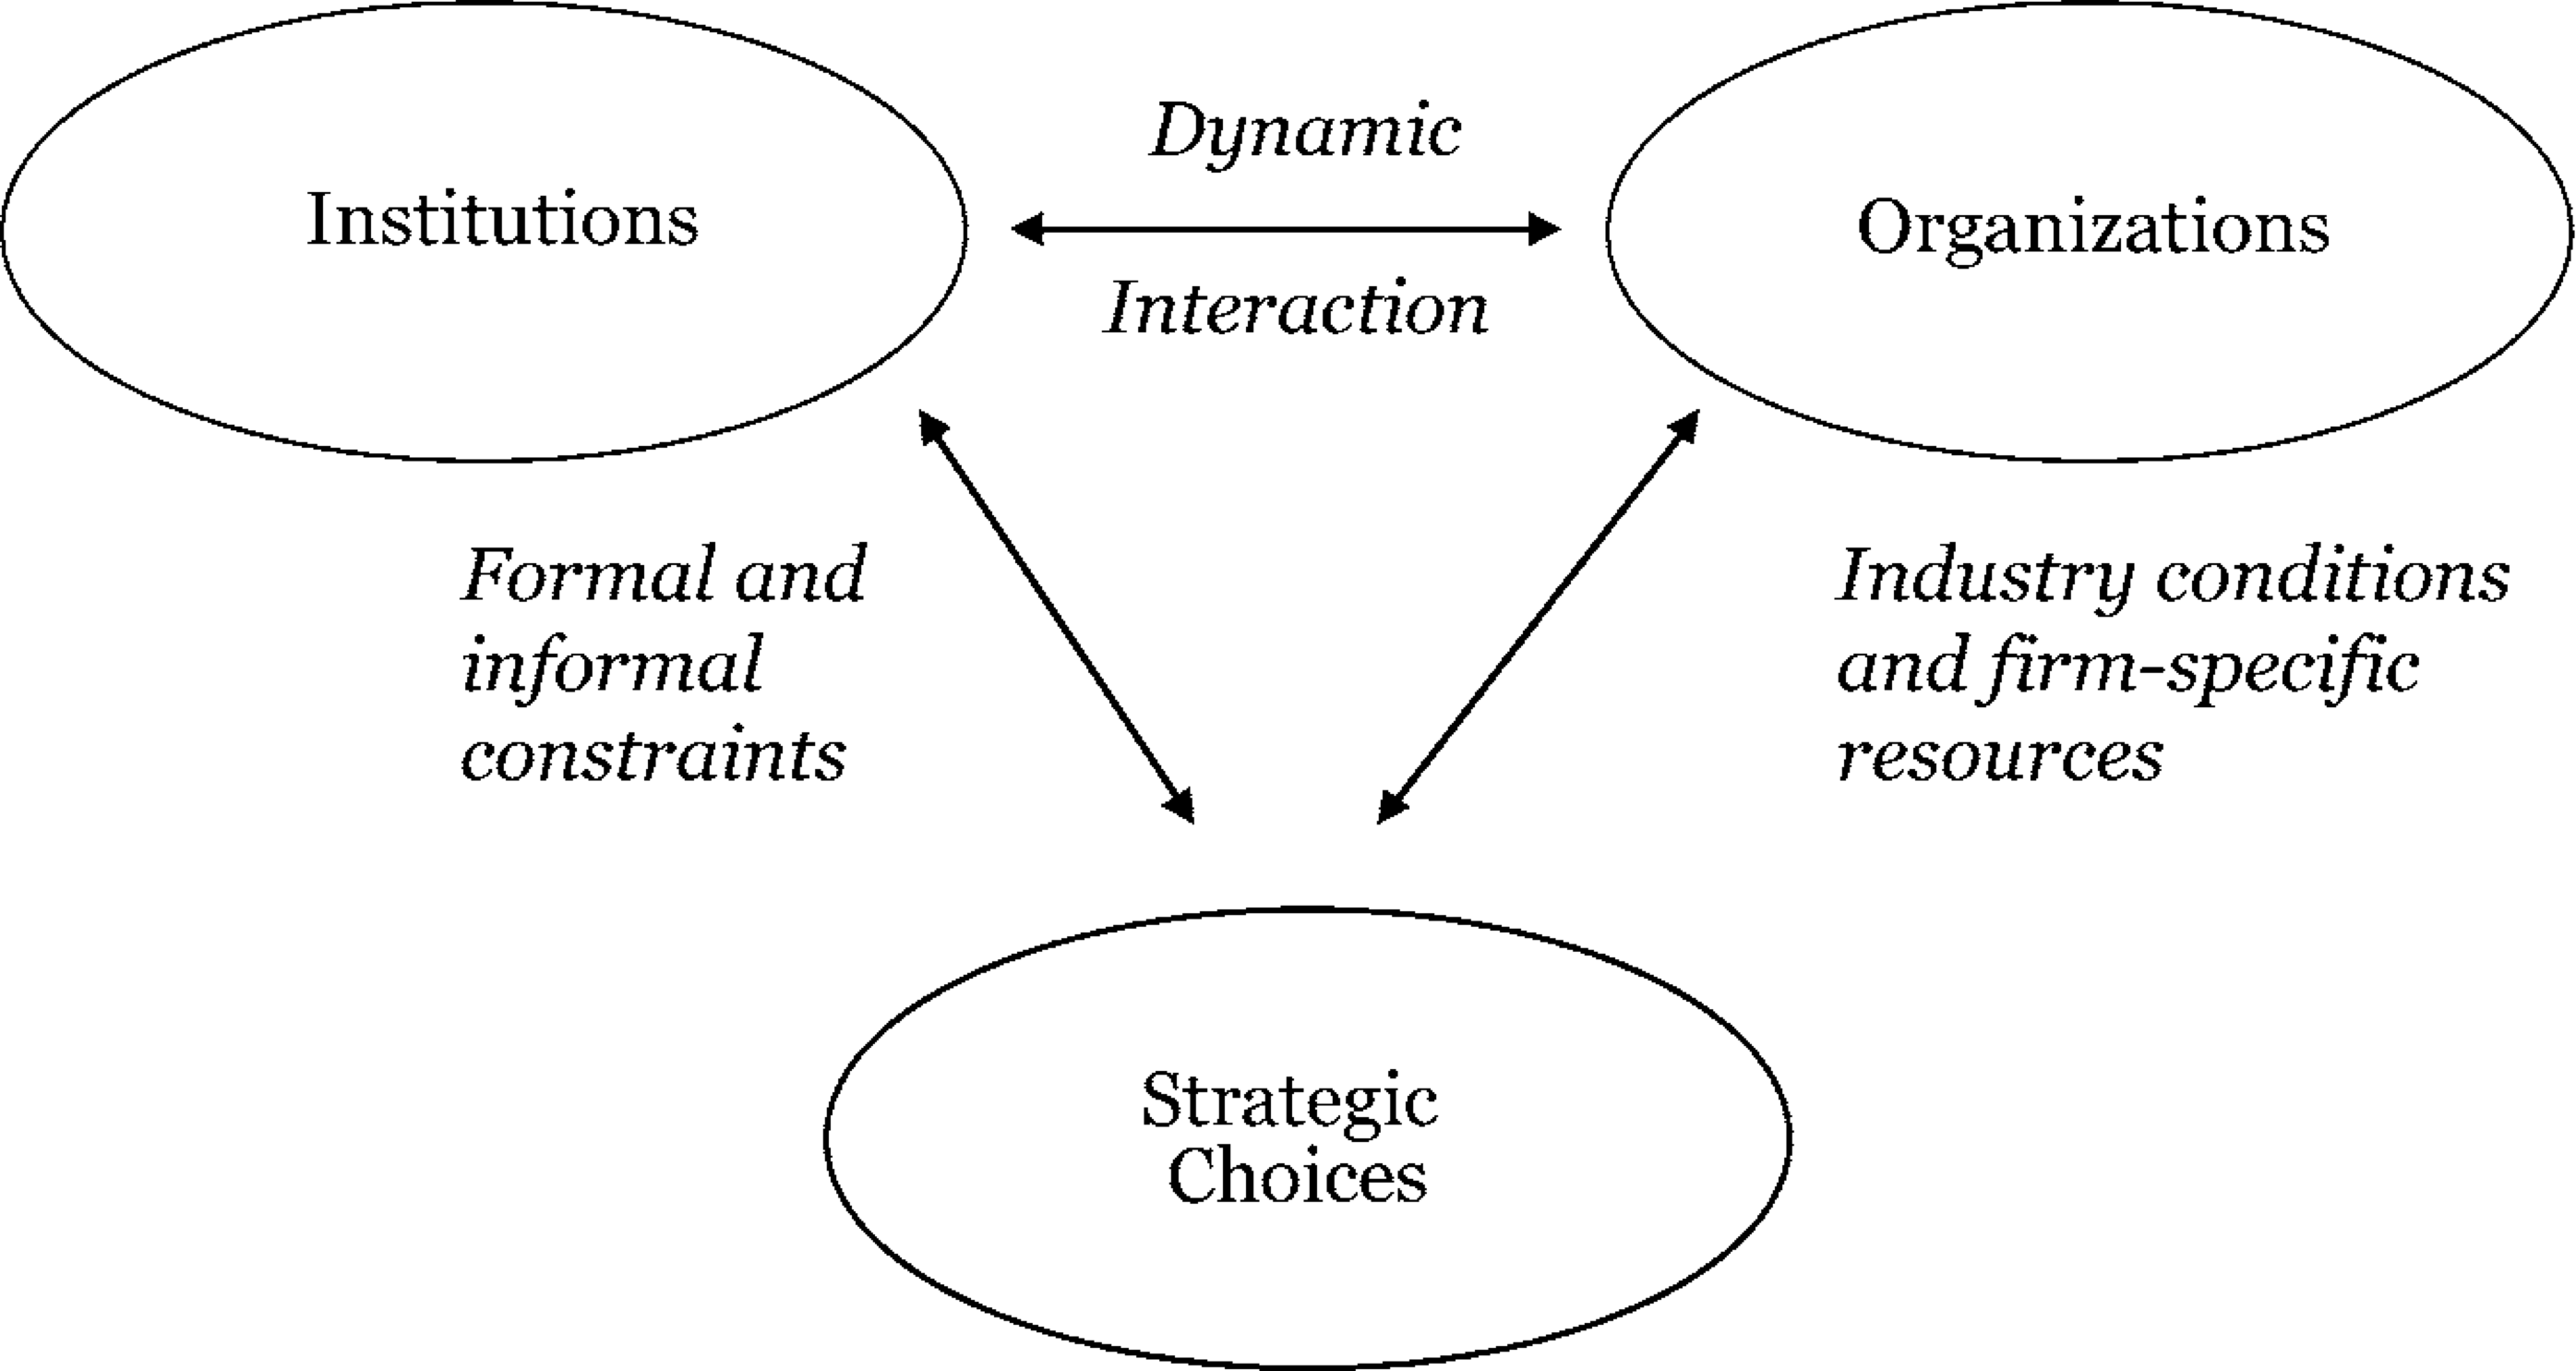
\includegraphics[width=0.65\textwidth]{IBV.pdf}
 	\caption{Institutions, organisations, and strategic choices. Source: \cite{Peng:2000}}
	\label{fig:ibv}
\end{figure}



Following~\cite{North:1990}, we understand institutions as ``humanly devised constraints
that structure human interaction". Institutional factors function as the formal and
informal ``rules of the game'' that socially constrain contracting practices between the \gls{BoD} and 
executives (\cite{North:1990}).
These formal en informal constraints operate in structures for both social and economic exchanges. 
Institutions are pervasive in that they are capable of shaping the behaviours of multiple actors (i.e. 
individuals, firms, industries, and~\glspl{NGO}). More broadly speaking, institutions serve to reduce 
uncertainty for different actors by conditioning the ruling norms of firm behaviours and defining the 
boundaries of what is considered legitimate.~\cite{Peng:2008}\\

So~\ibv~is cannot consist by itself but needs \rbv~\cite{Barney:1991} and \cite{Porter:1980} as is shown in figure~\ref{fig:ibv}. 
Where \rbv looked solely at the firm in a set environment \ibv also takes the surroundings into account. These surroundings are the institutions that govern the environment the \mne is playing the game. 
The actions of institutions can be divided into three pillars. Compliance from the firms occurs through \\(1) expedience (regulative pillar or coercive \iso),\\
 (2) social obligation (normative pillar or normative \iso), or \\
 (3) on a taken for granted basis (cognitive pillar) or mimetic \iso~where organisations respond to uncertainty by adopting patterns of other organisations that are deemed `successful'\cite{Westney:2005,Peng:2008,Kostova:1999,DiMaggio:1983,Scott:1995}.\\ 
\mne conform to these pillars or isomorphisms because these provide legitimacy~\cite{Powell:1991}

Although firms take decisions on the individual resources and capabilities \cite{Barney:1991} the influence of institutions can no longer be ignored. This is the difference between~\rbv and~\ibv. 

According to~\cite{Peng:2003} unfortunately, little is known about how organisations make strategic choices when confronting such large-scale institutional transitions.

\section{Institutional Theory}

 Firms do not only have to look at their resources and capabilities~\cite{Barney:1991}, but have to look at ``the rules of the game''~\cite{Scott:1995}. These so called rules include the environment that the firm \mne~has to adhere to.\\


Not only have   more scholars have come to realise that institutions matter~\cite{Powell:1991,Scott:1995}, and that strategy research cannot just focus on industry conditions and firm resources.\\

The central argument is that “organisations conform to the rules and beliefs systems in the environment because this isomorphism (regulatory, cognitive and normative) earns them legitimacy.

Not only have more scholars have come to realise that institutions matter and, that strategy research cannot just focus on industry conditions and firm resources alone~\cite{Powell:1991,Scott:1995}.

Nowadays institutional theory appears to be a highly insightful approach when probing into organisational strategies in Asia~\cite{Hoskisson:2000}.

\Gls{IB} has long been a favourite topic in academic literature. The term \gls{IB} alone gives over 2M hits in Google Scholar. Since~\cite{Porter:1980} introduced the concept of favourable industries, 

When introduced the \gls{RBV} in international business literature this view gained a lot of support. 
The theory has been expanded upon and \gls{IBV} was introduced by~\cite{Kostova:1999,Meyer:2009,Wang:2012}.


\section{}

